% Created 2017-02-12 Sun 23:09
% Intended LaTeX compiler: pdflatex
\documentclass[a4paper,11pt]{article}
\usepackage[utf8]{inputenc}
\usepackage[T1]{fontenc}
\usepackage{graphicx}
\usepackage{grffile}
\usepackage{longtable}
\usepackage{wrapfig}
\usepackage{rotating}
\usepackage[normalem]{ulem}
\usepackage{amsmath}
\usepackage{textcomp}
\usepackage{amssymb}
\usepackage{capt-of}
\usepackage{hyperref}
\usepackage[margin=1in]{geometry}
\usepackage{setspace}
\onehalfspacing
\usepackage{parskip}
\usepackage{amsthm}
\usepackage{amsmath}
\usepackage{mathtools}
\usepackage{hyperref}
\usepackage{graphicx}
\usepackage{tabularx}
\usepackage{booktabs}
\hypersetup{colorlinks,citecolor=black,filecolor=black,linkcolor=black,urlcolor=black}
\newtheorem{definition}{Definition}
\newtheorem{theorem}{Theorem}
\newcommand{\dx}{\mathrm{d}}
\newcommand{\var}{\mathrm{Var}}
\newcommand{\cov}{\mathrm{Cov}}
\newcommand{\corr}{\mathrm{Corr}}
\newcommand{\pr}{\mathrm{Pr}}
\newcommand{\rarrowd}[1]{\xrightarrow{\text{ \textit #1 }}}
\DeclareMathOperator*{\plim}{plim}
\newcommand{\plimn}{\plim_{n \rightarrow \infty}}
\setcounter{secnumdepth}{1}
\author{Zheng Tian}
\date{}
\title{Lecture 1: What is Econometrics?}
\hypersetup{
 pdfauthor={Zheng Tian},
 pdftitle={Lecture 1: What is Econometrics?},
 pdfkeywords={},
 pdfsubject={},
 pdfcreator={Emacs 25.1.1 (Org mode 9.0.3)}, 
 pdflang={English}}
\begin{document}

\maketitle
\setcounter{tocdepth}{1}
\tableofcontents


\section{What is Econometrics?}
\label{sec:org92a8322}

\subsection*{Definition of Econometrics}
\label{sec:orgbd4080a}

Econometricians may give you very different answers for the question
of \emph{What is Econometrics}. The following answers are all right from
their respective point of views:
\begin{itemize}
\item econometrics is the science of testing economic theories;
\item it is the set of tools used to forecasting future values
of economic variables;
\item it is the process of fitting mathematical economic model
to real-world data;
\item it is the science and art of using historical data to make
quantitative policy recommendations in government and business.
\end{itemize}

Stock and Watson (2015) define Econometrics as
\begin{quote}
At a broad level, econometrics is the science and art of using
economic theory and statistical techniques to analyze economic
data.
\end{quote}


\subsection*{Science or art?}
\label{sec:org22c764a}

Let us dissect the above definition a little bit. First, why is
econometrics the science AND art?

\begin{itemize}
\item Econometrics is a science because it essentially complies with the
principle of \textbf{falsifiability} of scientific research, as Karl Popper
defined. Figure \ref{fig:org1b84c2c} show a typical reasoning cycle
of a scientific research.\footnote{Source of Figure \ref{fig:org1b84c2c}: Martyn Shuttleworth (Sep
21, 2008). Falsifiability. Retrieved February 10th, 2017, from Explorable.com:
\url{https://explorable.com/falsifiability}.}

\begin{figure}[htbp]
\centering
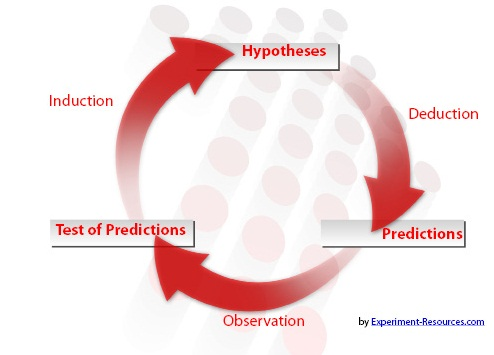
\includegraphics[width=0.6\textwidth]{figure/reasoning-cycle-research.jpg}
\caption{\label{fig:org1b84c2c}
A reasoning cycle of scientific research}
\end{figure}

Econometricians propose a hypothesis based on either existing economic
theories or their own economic reasoning, and then collect data to
test the hypothesis that can be rejected or fail to be rejected. Even
though an economic theory is not rejected by one set of data at a
time period, it can be very likely to be rejected using another set of
data at another time period. Then, a new theory or hypothesis will
be brought up.

\item Econometrics is an art because the data are usually incomplete and
unobserved to validate a hypothesis, so we need to use human
creativity to reach a balance between scientific rigor and realistic
approximation.
\end{itemize}

The following quote captures the dual nature of econometrics as both
science and art:
\begin{quote}
Econometrics is alchemy since econometricians can create nearly any
result desired, but it is also science because econometricians also
know how to reject and avoid spurious models. -- Hansen (1996)
\end{quote}


\subsection*{Economic theory, statistics, and data}
\label{sec:org499311f}

A complete process of econometric research inevitably consists of three
components: economic theory, statistical techniques, and economic
data. When we have a research question, we first need to find or
formulate an economic theory that can be either a formal mathematical
model or a logical economic reasoning. Guided with this economic
theory, we build an econometric model to characterize the relationship
between various variables involved in the theory. Then we collect data
to measure these variables, and use statistical techniques to estimate
the model and test hypotheses that are raised from the theory.

\begin{figure}[htbp]
\centering
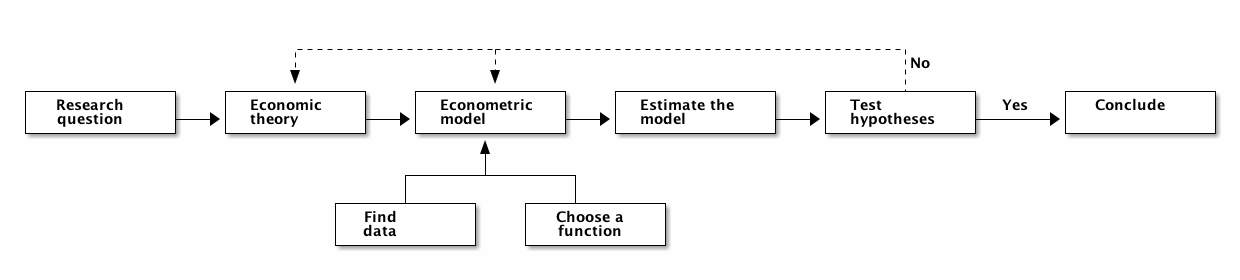
\includegraphics[width=1.0\textwidth]{figure/econometric_workflow.png}
\caption{\label{fig:orged9c2a8}
A workflow of econometric research}
\end{figure}

Let's look at a real example to get a first impression of what is
econometrics.


\section{Economic Questions We Examine}
\label{sec:org5afe1f9}

\subsection*{Question \#1: Does reducing class size improve elementary school education?}
\label{sec:org22cbe87}

\subsubsection*{The story goes like this}
\label{sec:org9870b40}

There is a proposal for improving basic learning in elementary schools
in the U.S. It suggests reducing class size, arguing that with fewer
students in the classroom, each students get more of the teacher's
attention, there are fewer class disruptions, learning is thus
enhanced, and grades improve. Researchers want to find evidence to
prove such arguments.

\subsubsection*{The question of interest}
\label{sec:org39ea275}

The question of interest in this example is whether there is
any effect of reducing class size on improving students' grades in
elementary schools.

Before we start a research project, we often consider its practical
significance. Simply, who will care such a research? We could list
parents, school principles, superintendents of school districts,
school board  members, and the list goes no, who are at stake with
such a research project.

\subsubsection*{The research design}
\label{sec:orgf466c71}

To investigate the effect of class size on learning performance, we
can do either qualitative research or quantitative research. A field
study, for example, is a qualitative research in which researchers
will interview students and teachers and follow some classes for a
period on the spot. Although qualitative research design is not the focus of
this course, we should keep in mind of such a research direction.

We focus on a quantitative research design because we want to know
exactly how much improvement in students' learning would be when class
size is reduced by one student per class. Researchers use \textbf{randomized
controlled experiments (RCE, or randomized controlled trial, RCT)} to
examine the magnitude of the effect. We will explain RCE in the next
section.

\subsubsection*{The sample and data}
\label{sec:org0c461ce}

Obviously, it is unfeasible to carry out such an experiment
nationwide. So researchers draw samples and collect data from 420
California school districts in 1999. We will use this California
school dataset throughout this course. So let's take a glimpse. Figure
\ref{fig:org607a030} is a screen shot of the first 25 observations in the
dataset.

\begin{figure}[htbp]
\centering
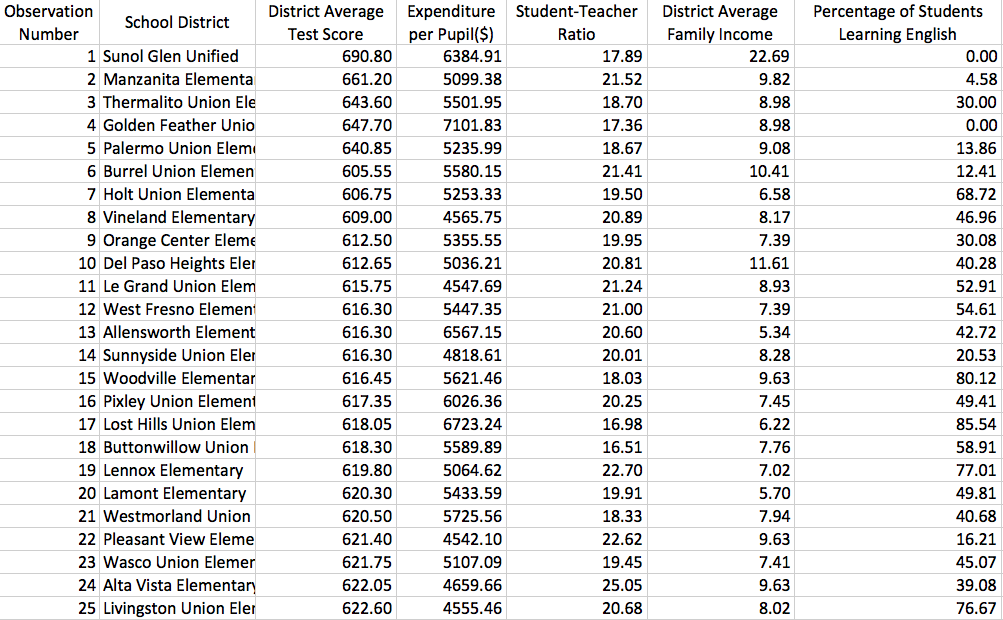
\includegraphics[width=1.0\textwidth]{figure/table1_1.png}
\caption{\label{fig:org607a030}
A screen shot of the dataset the California school districts in 1999}
\end{figure}

This is an example of cross-sectional data. Each row represents a
distinct unit of observation, which is a school district in California
in this example. All observations are collected in a single
year. Although an observation number is assigned to each row, the
order bears no real meaning, that is, the sorting of observations is
arbitrary. Having the data in hand, the next step is to set up an
econometric model.

\subsubsection*{The econometric model}
\label{sec:orgfcf86d3}

Since there is no formal economic theory underlying this research, we
use our common sense to build an econometric model. The key variables
involved in this research is the performance of students' learning and
class size. The former is measured by the average test scores in a
school district (\emph{TestScore}), and the latter is measured by student-teacher
ratios (\emph{STR}). For simplicity, we set up a \textbf{simple linear regression
model} as follows,

\[ TestScore = \beta_0 + \beta_1 STR + OtherFactors  \]

The hypothesis we make is that if \emph{STR} has a non-zero effect on
\emph{TestScore}. The model is then estimated using some estimation method,
and we test the hypothesis with the estimation results using some test
statistics. All of these comprise the core of this course.


\subsection*{Three other questions}
\label{sec:org9c40033}

Chapter 1 in The textbook explaines three other questions that can be
answered using different types of data and applying different
econometric methods.

\begin{description}
\item[{Question 1}] Does reducing class size improve elementary school education?
\item[{Question 2}] Is there racial discrimination in the market for home loan?
\item[{Question 3}] How much do cigarette taxes reduce smoking?
\item[{Question 4}] What will the rate of inflation be next year?
\end{description}

\begin{table}[htbp]
\caption{\label{tab:orga6aeec4}
Data types and econometric methods for all four questions}
\centering
\begin{tabular}{lll}
Questions & Data types & Econometric methods\\
\hline
\#1 & experimental, cross-sectional & multiple regression\\
\#2 & observational, cross-sectional & multiple regression with binary dependent variable\\
\#3 & observational, panel data & Panel data regression model\\
\#4 & observational, time series & multiple regression with lagged dependent variable\\
\end{tabular}
\end{table}


\section{Causal Effects and Idealized Experiments}
\label{sec:orgcb63cd1}

In the example of California School districts, the main concern of the
research is whether reducing class size would improve students'
learning, comprising a \textbf{causal relationship} between reducing class
size (the cause) and improvement in test scores (the consequence). To
disentangle from other factors that could influence test scores,
researchers conduct a randomized controlled experiment. 

\subsection*{Randomized controlled experiment}
\label{sec:org14671f6}

Randomized controlled experiments (or trials, RCT thereafter) are
commonly used in clinical trial to test the effectiveness of medical
intervention. In a randomized controlled experiment, the participants
are randomly assigned to two groups: a control group and a treatment
group. The control group receives no treatment (or placebo), while the
treatment group receives the treatment. After a follow-up period,
researchers compare the two groups to check the effectiveness of the
treatment. See an illustration of RCTs in Figure \ref{fig:orgd2cc4d5}. \footnote{Source of Figure \ref{fig:orgd2cc4d5}: Emma Tomkinson (May 20,
2013). Retrieved February 12th, 2017, from
\url{https://emmatomkinson.com/2013/05/20/randomised-controlled-trials-rcts-in-public-policy/}.}

\begin{figure}[htbp]
\centering
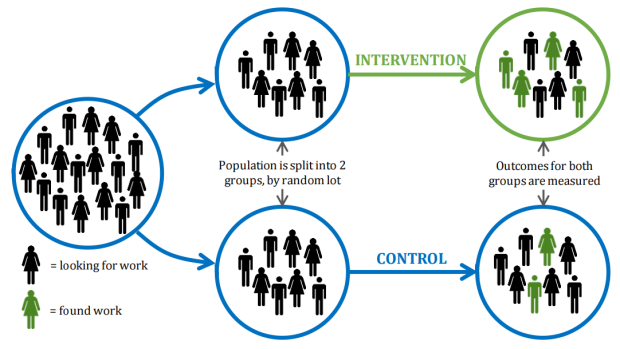
\includegraphics[width=1.0\textwidth]{figure/rct_example.png}
\caption{\label{fig:orgd2cc4d5}
An illustration of a randomized controlled experiment}
\end{figure}

The most important advantage of RCT is that randomization minimizes
selection bias and the different comparison groups allow the
researchers to determine any effects of the treatment when compared
with the no treatment (control) group, while other variables are kept
constant.\footnote{Randomized controlled trial. In \emph{Wikipedia}. Retrieved February
12th, 2017, from
\url{https://en.wikipedia.org/wiki/Randomized\_controlled\_trial}.} In the example of California school districts,
randomized control experiments ensure that the only systematic difference
between the classes in the control group and those in the treatment
group is the treatment (reduced class size) itself, with the effects
from other \textbf{confounding factors} eliminated. 

However, there are the disadvantages of RCTs. Among the most
frequently cited drawbacks are:
\begin{description}
\item[{Time and costs}] RCTs usually are expensive to undertake and take a
long time to observe the effect of treatment.
\item[{Conflict of interest dangers}] RCTs may be funded by special interest
groups so that its objectivity is doubtful.
\item[{Ethnics}] Especially in social science, we cannot impose some
treatment due to ethnic concerns.
\end{description}


\subsection*{Causal effect}
\label{sec:org9df9ca4}

\textbf{Causal effect} is defined to be the effect on an outcome of a given
action or treatment as measured in an ideal RCT. Although it is almost
impossible to do an ideal RCT, the concept of the ideal randomized
controlled experiment does provide a theoretical benchmark to define
causal effects in research design, while the implementation of such an
experiment is nearly impossible. Most econometric methods to be taught
in this course concern detecting the causal effect among variables. 


\section{Data Sources and Types}
\label{sec:orgdb98e7d}

\subsection*{Experimental versus observational data}
\label{sec:org0c1088c}

\textbf{Experimental data} come from experiments designed to evaluate a
treatment or policy or to investigate a causal effect. \textbf{Observational
(or nonexperimental) data} are collected using surveys, and
administrative records.

The problem of using observational data to estimate causal effects is
that the "treatment" is not randomly assigned, so it is challenging to
sort out the effect of the "treatment" from other relevant
factors. Much of econometric methods are developed to deal with
causality using observational data.


\subsection*{Cross-sectional data}
\label{sec:orgf0df436}

Data on different entities for a single time period are called
\textbf{cross-sectional data}. The sequence of each observation number is
arbitrarily assigned. The data in the example of California school
districts are cross-sectional. Cross-sectional data can be
experimental data or observational data. 


\subsection*{Time series data}
\label{sec:org3d52383}

Time series data are data for a single entity collected at multiple
time periods. The sequence of each record is based on the time period
it happened, which bears real meaning in understanding the trend. An
example of time series data is the consumer price index (CPI) of China
by month from 1990 to 2014. Most time series data are
observational. This course will not cover any chapters regarding time
series data, but it will be another course in our econometric series. 


\subsection*{Panel data}
\label{sec:org9e04857}

\textbf{Panel data}, also called \textbf{longitudinal data}, are data for multiple
entities in which \textbf{each entity} is observed at two or more time
periods. Panel data are very useful for estimating causal effects. If
time permits, we will cover some basic use of panel data at the end of
this course. 
\end{document}